\begin{figure}
	\centering
	\begin{subfigure}{0.48\linewidth}
		\centering
		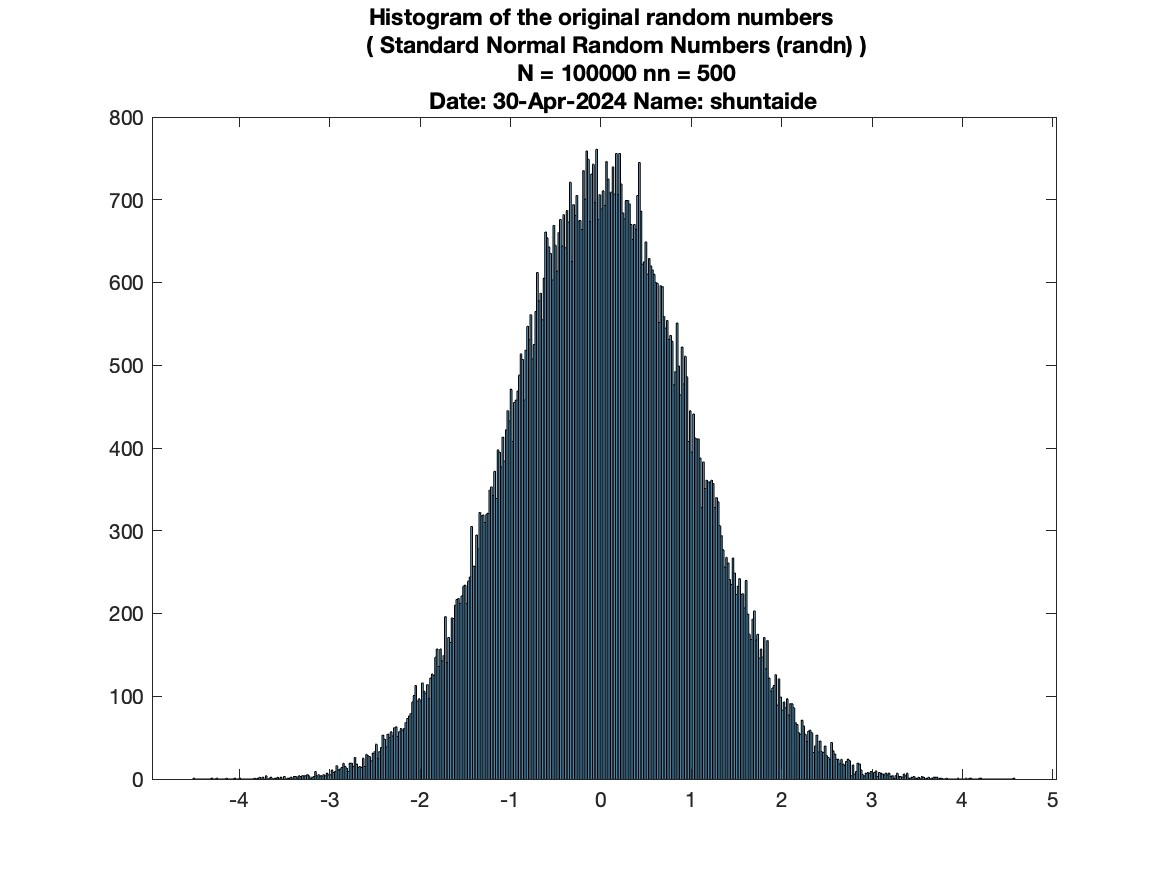
\includegraphics[width=0.8\textwidth]{src/figures/cl-standard-normal/cl_original_randn_hist_N=100000_nn=500.jpg}
		\subcaption{元々の分布}\label{fig:cl-standard-normal-original}
	\end{subfigure}
	\begin{subfigure}{0.48\linewidth}
		\centering
		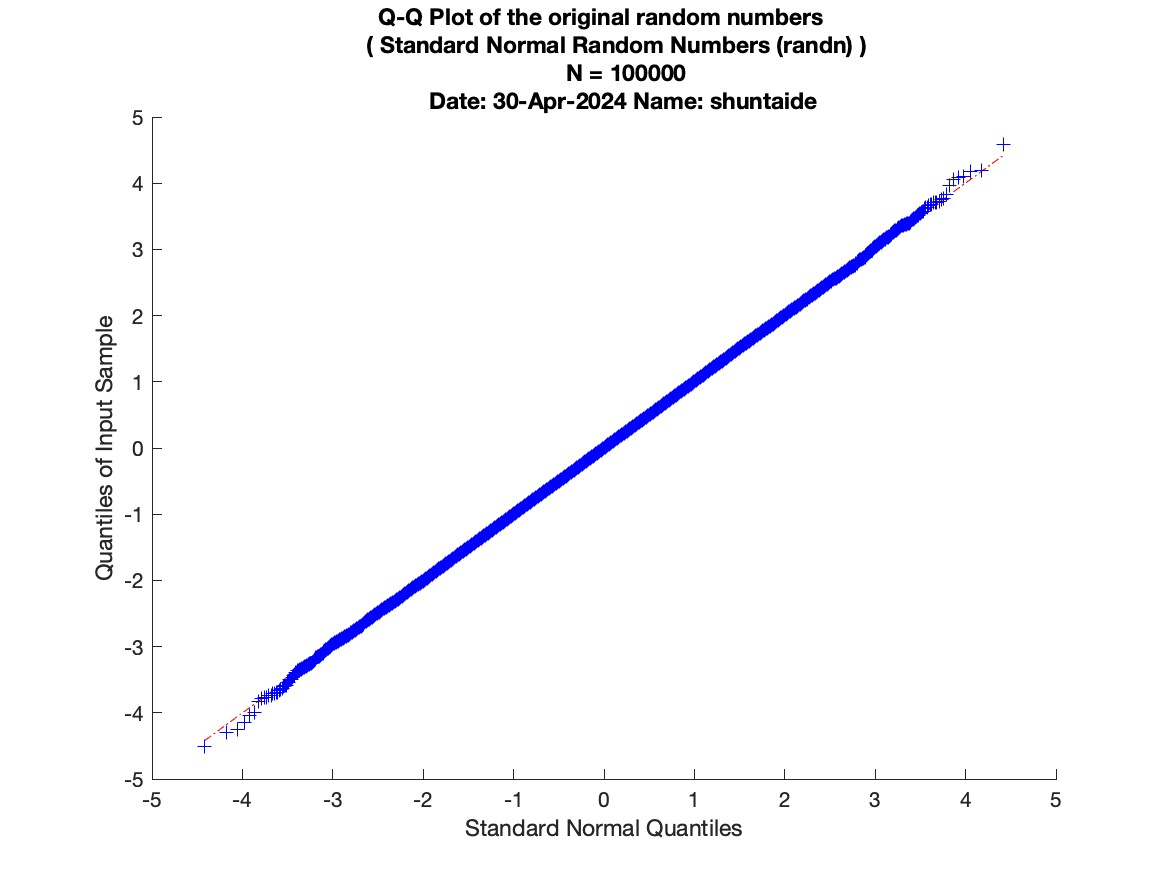
\includegraphics[width=0.8\textwidth]{src/figures/cl-standard-normal/cl_original_randn_qqpl_N=100000.jpg}
		\subcaption{元々の分布のQQプロット}\label{fig:cl-standard-normal-original-qqpl}
	\end{subfigure}
	\begin{subfigure}{0.48\linewidth}
		\centering
		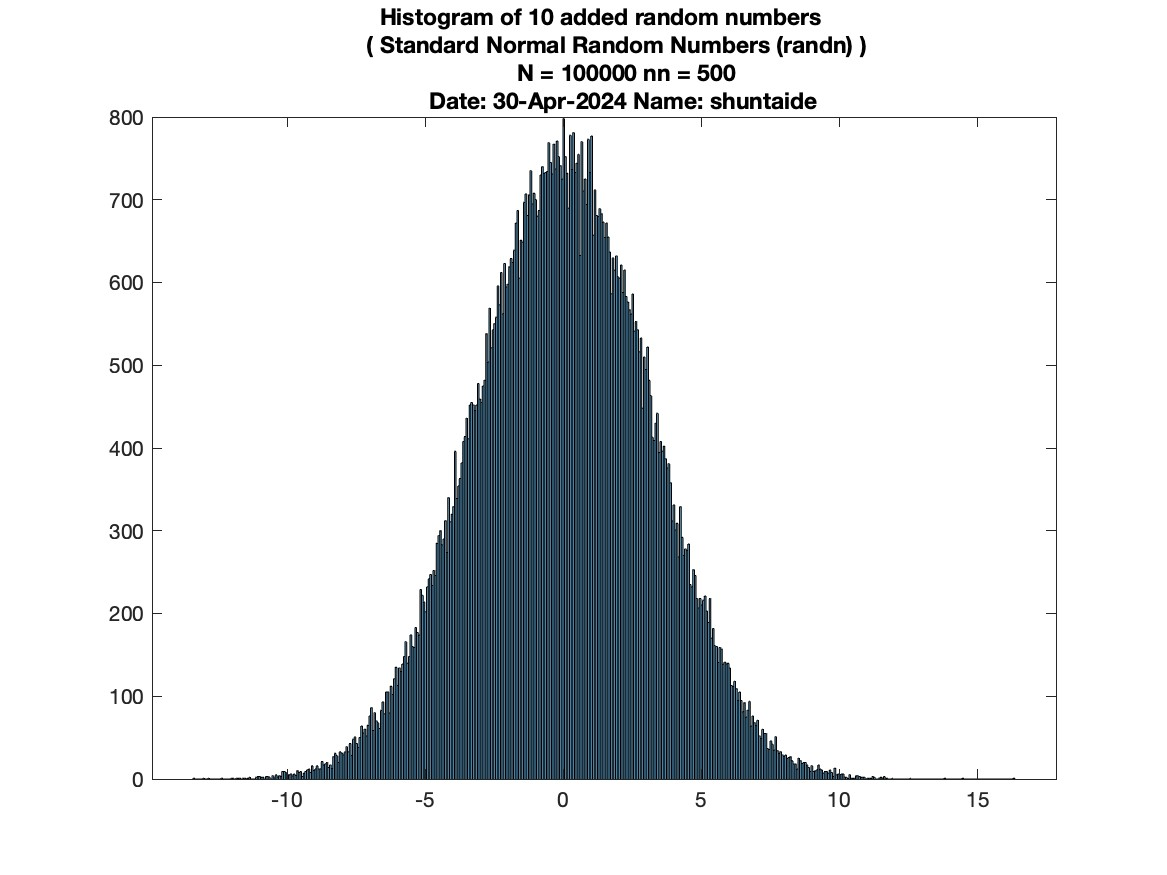
\includegraphics[width=0.8\textwidth]{src/figures/cl-standard-normal/cl_added_randn_hist_N=100000_nn=500.jpg}
		\subcaption{加算した場合の分布}\label{fi:cl-standard-normal-added}
	\end{subfigure}
	\begin{subfigure}{0.48\linewidth}
		\centering
		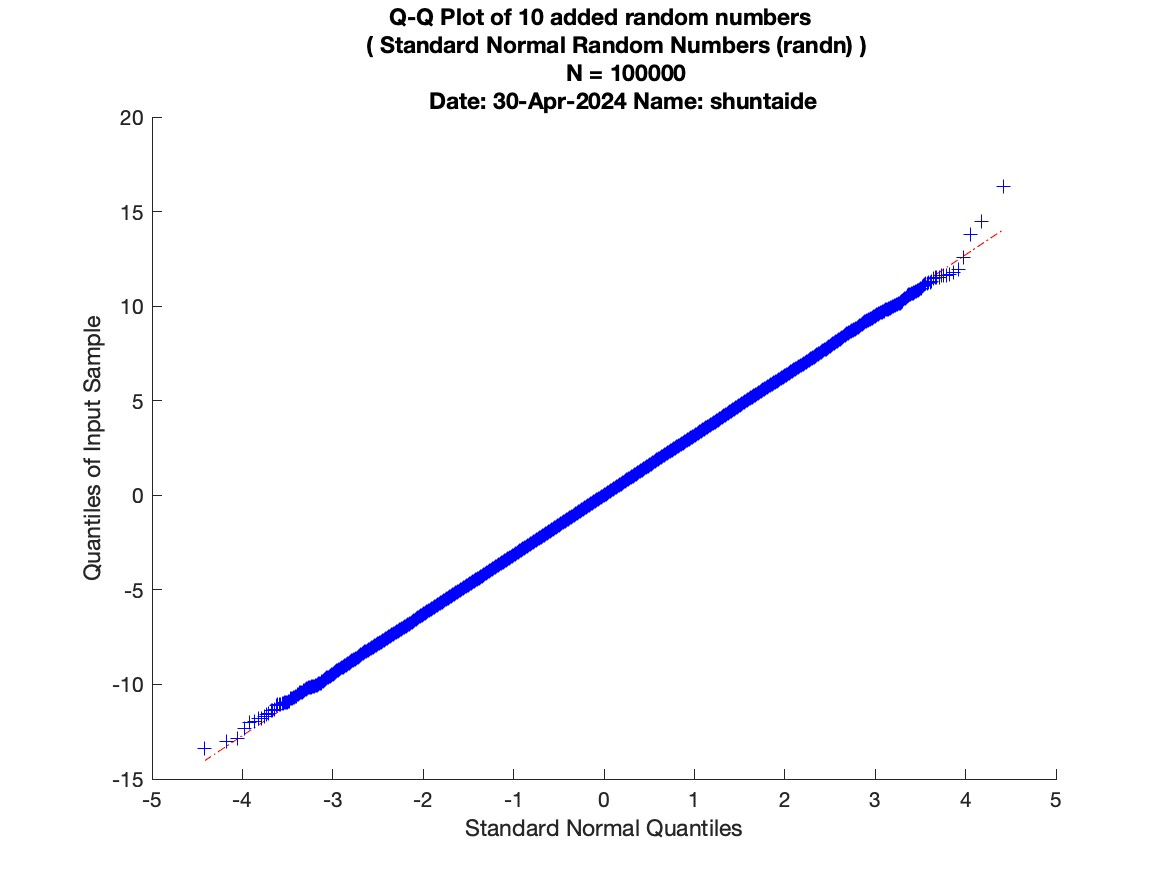
\includegraphics[width=0.8\textwidth]{src/figures/cl-standard-normal/cl_added_randn_qqpl_N=100000.jpg}
		\subcaption{加算した場合のQQプロット}\label{fig:cl-standard-normal-added-qqpl}
	\end{subfigure}
	\caption{標準正規乱数による生成結果}\label{fig:cl-standard-normal-random}
\end{figure}
